\documentclass[preprint,12pt]{elsarticle}
\usepackage{graphicx}
\usepackage{amssymb}

\journal{CS4701 - Bart Selman}

\begin{document}

\begin{frontmatter}
	\title{3D Tic-Tac-Toe}
	\author{Lillian Chen (qc53) \& Jim Yu (jly29)}
	\address{Cornell University}

	\begin{abstract}
		In the interest of exploring the subject of game trees, we have implemented a 3-dimensional tic-tac-toe game and an artificial intelligent player in python. This paper will include a clear description of the overall goals of the project, the software written, and the results an evaluation of our system with various observations on the AI components and their performance.
	\end{abstract}
\end{frontmatter}

\section{Game Analysis}
	3D tic-tac-toe is a two player game that slightly modifies the rules of the original tic-tac-toe game by presenting a different board setup. Rather than one 3x3 board where players X and O can each place their moves, 3D Tic-tac-toe essentially has three 3x3 boards on top of each other such that the method to win now changes. (Note, however, that the center tile of the middle board is an invalid space. More on this in Section 1.1.) The goal of the game is still to reach three respective marks in a row but now this row can line up vertically, horizontally, or diagonally on either a single board or across all three.

	\subsection{Play Mechanics}
		Upon initiation, the game begins at the menu, where there are three buttons: play, learn, and about. The about option is a simple text screen giving brief credits and information about the project.

		The play option (Figure 1) is the human versus computer mode, the former represented by an X and the latter an O. The human player is given a prompt prior to starting the game to choose whether he would like to make the first move. The game then begins and displays three 3x3 boards representing the top, middle, and bottom board in that order. Depending on the player's earlier choice, an O, representing the computer's move, will be on the board. At this point, the human player is free to use the mouse and click on a tile for his own move. All inputs outside of a tile, on the center tile of the middle board, or on a tile already chosen by either player are invalid and will not be registered. This repeats until some player achieves 3 consecutive marks in a row and wins, after which the human player is directed back to the menu.

		The learn option is essentially the same as the play mode but the computer plays against itself in order to fill its game tree data further. Games between the computer players will repeat until prompted to stop, therefore allowing the program to be left alone for an extended period of time to reach an optimal AI player.

		\begin{figure}[h]
			\centering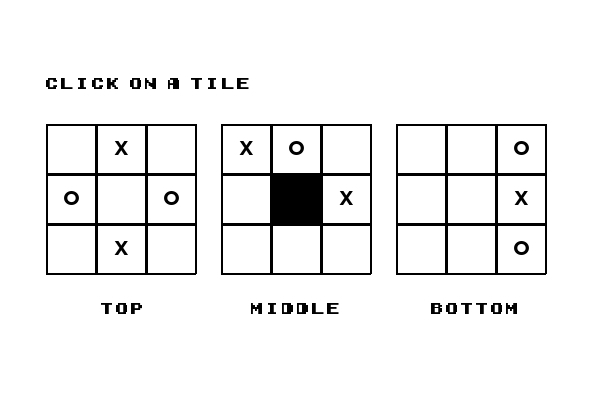
\includegraphics[width=0.5\linewidth]{1.jpg}
			\caption{Figure 1: play mode displaying top, middle, bottom boards}
		\end{figure}

	\subsection{Omission of Center Tile}
		The choice to leave out the center tile on the middle board was made in order to avoid an extreme advantage given to the player who chooses to take the space.

		If the center tile was not omitted, there would be 49 distinct 3-in-a-rows, given that there are 8 on each board, 9 vertically stacked columns, and 16 diagonally configured rows stretching across all three boards. Of these, there are 12 rows that include the center tile, making them approximately a quarter of the winning rows. Therefore, if the first player takes this space, he will be eliminating a quarter of the possible positions to win for his opponent.

		However, the higher worry is that an intelligent human player can take advantage of the board to force a win for himself regardless of the actions of the opponent. The strategy for this win can span as little as 7 total actions because given the prompt to make the first move, the human can respond yes and immediately occupy the center tile. Then, whichever tile the AI chooses, the human can respond with a move that forces the AI to counter it in its next turn. Very soon, there will reach a point where there are more than one spaces for the human player to win and the AI not being able to block all of them in one turn will be ensured a loss. With this strategy in place then, the computer will have no chance with or without artificial intelligence, rendering the purpose of this project moot.

		Of course, if the human player is unaware of this winning strategy, the computer can also take advantage of it without meaning to do so. This is because as the AI fills its game tree, it can easily find the routes corresponding to this strategy as the goal state is reached at 7 moves. And with the guaranteed victory of these series of steps, the AI that we implemented will always take the move leading to the outcome with the highest history of wins, therefore influencing the computer over time to utilize this strategy without ever having known about it.

		For this reason, we have omitted the center tile in order to test the full ability of our AI player without taking advantage of the board itself. We believe this will allow us to explore the depths of our subject further and fulfill our intended goal in a more meaningful way.

	\subsection{Resolving Ties}
		THERE ARE NONE

\section{The Second Section}
	\label{S:2}

	Etiam congue sollicitudin diam non porttitor. Etiam turpis nulla, auctor a pretium non, luctus quis ipsum. Fusce pretium gravida libero non accumsan. Donec eget augue ut nulla placerat hendrerit ac ut mi. Phasellus euismod ornare mollis. Proin tempus fringilla ultricies. Donec pretium feugiat libero quis convallis. Nam interdum ante sed magna congue eu semper tellus sagittis. Curabitur eu augue elit.

	Aenean eleifend purus et massa consequat facilisis. Etiam volutpat placerat dignissim. Ut nec nibh nulla. Aliquam erat volutpat. Nam at massa velit, eu malesuada augue. Maecenas sit amet nunc mauris. Maecenas eu ligula quis turpis molestie elementum nec at est. Sed adipiscing neque ac sapien viverra sit amet vestibulum arcu rhoncus.

	Vivamus pharetra nibh in orci euismod congue. Pellentesque habitant morbi tristique senectus et netus et malesuada fames ac turpis egestas. Quisque lacus diam, congue vel laoreet id, iaculis eu sapien. In id risus ac leo pellentesque pellentesque et in dui. Etiam tincidunt quam ut ante vestibulum ultricies. Nam at rutrum lectus. Aenean non justo tortor, nec mattis justo. Aliquam erat volutpat. Nullam ac viverra augue. In tempus venenatis nibh quis semper. Maecenas ac nisl eu ligula dictum lobortis. Sed lacus ante, tempor eu dictum eu, accumsan in velit. Integer accumsan convallis porttitor. Maecenas pretium tincidunt metus sit amet gravida. Maecenas pretium blandit felis, ac interdum ante semper sed.

	In auctor ultrices elit, vel feugiat ligula aliquam sed. Curabitur aliquam elit sed dui rhoncus consectetur. Cras elit ipsum, lobortis a tempor at, viverra vitae mi. Cras sed urna sed eros bibendum faucibus. Morbi vel leo orci, vel faucibus orci. Vivamus urna nisl, sodales vitae posuere in, tempus vel tellus. Donec magna est, luctus non commodo sit amet, placerat et enim.

\end{document}